\documentclass{article}

% Language setting
% Replace `english' with e.g. `spanish' to change the document language
\usepackage[english]{babel}

% Set page size and margins
% Replace `letterpaper' with `a4paper' for UK/EU standard size
\usepackage[a4paper,top=2cm,bottom=2cm,left=3cm,right=3cm,marginparwidth=1.75cm]{geometry}

% Useful packages
\usepackage{amsmath}
\usepackage{graphicx}
\usepackage[colorlinks=true, allcolors=blue]{hyperref}

\usepackage{placeins}

\usepackage{pifont}
\newcommand{\cmark}{\ding{51}} % ✓
\newcommand{\xmark}{\ding{55}} % ✗

\usepackage{tikz}
\usetikzlibrary{arrows.meta,positioning,shapes.geometric}

\usepackage{subcaption}
\usepackage{booktabs}
% \title{Your Paper}
% \author{You}


 \begin{document}
 

\FloatBarrier
\section{Introduction}

The objective of the MaCFP-4 solid-phase modelling exercise was to focus initially on model-to-model comparisons. The material selected for this study is pine wood, investigated under anaerobic conditions. Combustion and oxidation phenomena are deliberately excluded from the present exercise, as they will be addressed in the subsequent MaCFP-5 benchmark.

In line with this objective, participants are requested to perform TGA and FPA simulations under the operating conditions described in Table~\ref{tab:studied_scenarios}.

\begin{table}
\centering
\begin{tabular}{c|c|c}
                                   & \textbf{TGA}         & \textbf{FPA} \\\hline
\textbf{Heating rate or Heat flux} & 10 K/min ; 100 K/min & 10 kW/m² ; 30 kW/m² ; 60 kW/m²\\
\textbf{Thickness (mm)}            & -                    & 6 ; 18 
\end{tabular}
\caption{\label{tab:studied_scenarios}Summary of the studied scenarios.}
\end{table}

Consequently, the TGA part of the benchmark comprised two simulation cases, while the combination of two sample thicknesses and three external heat fluxes led to six FPA scenarios to be simulated. For the one-dimensional FPA simulations, an adiabatic boundary condition was imposed on the rear surface of the sample, and no convection was considered on the exposed surface.

With regard to the modelling approach, no specific physical assumptions were prescribed. The intention was to provide participants with the freedom to configure their models and select assumptions based on their own expertise and modelling practices.

To perform this phase of the modelling exercise, participants required input data in the form of kinetic parameters and thermophysical properties. Modelers were free to use experimental data generated by any participant in the associated experimental benchmark exercise \textcolor{red}{(section REF)}, to perform their own parameter calibrations, or to adopt a combination of both approaches (or even complete the data set from literature). It should be noted that the calibration of kinetic and thermophysical parameters constituted an integral part of the benchmark exercise, and the resulting methodologies and outcomes are discussed separately in \textcolor{red}{(section REF)}.

\section{Participating organizations}

A total of four submissions were received in this benchmark exercise. Two of these submissions resulted from collaborations between two organizations, leading to the following four participating teams:

\begin{itemize}
    \item \textbf{CORIA} (Complexe de Recherche Interprofessionnel en Aérothermochimie) -- France;
    
    \item \textbf{FSRI--UMD}, a collaboration between the Fire Safety Research Institute and the University of Maryland -- USA;
    
    \item \textbf{NIST--StMU}, a collaboration between the National Institute of Standards and Technology and Saint Mary's University -- USA;
    
    \item \textbf{UCB} (University of Colorado Boulder) -- USA.
\end{itemize}

Table~\ref{tab:organization_scenarios} summarizes the scenarios modelled by the participating organizations. All organizations simulated the full set of scenarios, except NIST-StMU, which submitted simulations for the TGA scenarios only.

\begin{table}
\centering
\begin{tabular}{c|c|c|c|c}
                & \textbf{CORIA}         & \textbf{FSRI - UMD} & NIST-StMU  & UCB     \\\hline
\textbf{0D TGA} & \cmark                 & \cmark              & \cmark     & \cmark  \\
\textbf{1D FPA} & \cmark                 & \cmark              & \xmark     & \cmark
\end{tabular}
\caption{\label{tab:organization_scenarios}Simulated scenarios by the participating organizations.}
\end{table}

\section{Model description}

This section is intended to provide a brief description of the physical assumptions adopted by the different participating organizations when developing their respective models. A detailed description of these assumptions can be found in the dedicated MaCFP-4 repository (see. \textcolor{red}{(repo link)}).

\subsection{CORIA modeling assumptions}

The pyrolysis process was represented by three parallel decomposition reactions corresponding to the three main wood pseudo-components, namely hemicellulose, cellulose, and lignin (Eq.~\ref{eq:CORIA-pyrolysis-reactions}). The initial mass fraction of these pseudo-components, are taken from literature \cite{marquezmontesino2021}: 0.163, 0.544 and 0.293, respectively. Dry wood was assumed in both the TGA and FPA simulations. The kinetic parameters were identified from TGA experiments from the MaCFP-4 experimental database (data set from laboratory UMET),  using the DAKOTA code and the NL2SOL optimization algorithm, and the resulting kinetic mechanism was subsequently employed in the FPA gasification simulations. Constant thermophysical properties, taken from the literature, were considered throughout the simulations. For the FPA configuration, fibers were assumed to be oriented perpendicular to the exposed surface. The gasification simulations were performed with the PATO code \cite{lachaud2017}. Radiative heat exchange was prescribed at the exposed surface, with no convection. A zero-temperature-gradient condition was imposed at the rear surface.

\begin{equation}
\label{eq:CORIA-pyrolysis-reactions}
\begin{aligned}
\mathrm{Cellulose}      &\rightarrow n_1\,\mathrm{char} + (1-n_1)\,\mathrm{gas} \\
\mathrm{Hemicellulose}  &\rightarrow n_2\,\mathrm{char} + (1-n_2)\,\mathrm{gas} \\
\mathrm{Lignin}         &\rightarrow n_3\,\mathrm{char} + (1-n_3)\,\mathrm{gas}
\end{aligned}
\end{equation}

%\begin{figure}
%\centering
%\includegraphics[width=0.25\linewidth]{frog.jpg}
%\caption{\label{fig:frog}This frog was uploaded via the file-tree menu.}
%\end{figure}


\subsection{FSRI - UMD modeling assumptions}

Two material property sets were considered: an optimized property set (\textbf{OPT}), relying primarily on inverse analysis, and a directly measured property set (\textbf{DM}), based as much as possible on experimentally measured properties. Both OPT and DM models employed the same thermal degradation kinetics and thermodynamics. The pyrolysis process was represented by six sequential first-order reactions, including one moisture evaporation reaction and five thermal degradation reactions. Kinetic and energetic parameters were calibrated against TGA and DSC measurements obtained at multiple heating rates. The kinetic parameters were identified from STA/TGA experiments conducted by FSRI at 3 and 30 K min$^{-1}$ and by UMD at 10 K min$^{-1}$ using a multi-stage hill-climbing optimization algorithm implemented in Julia and coupled with the \texttt{Pyrolysis.jl} model. The heats of reaction were subsequently calibrated against DSC measurements acquired at 10 K min$^{-1}$. For the FPA simulations, the models were implemented in FDS version 6.10.1 and neglected the moisture evaporation reaction. Temperature-dependent thermophysical properties were considered throughout the simulations. Specific heat capacities, densities, emissivities, and thermal conductivities were either directly derived from dedicated experiments (DM model) or identified through inverse analyses (OPT model). Surface emissivities were based on integrating-sphere measurements and depended on the incident heat flux, while radiation absorption was assumed to occur entirely at the exposed surface because of the high absorption coefficient of both virgin wood and char. \\

The contribution of FSRI - UMD represents two distinct models: the OPT model and DM one. Consequently, these two models will be refred to as \textbf{FSRI-UMD OPT} and \textbf{FSRI-UMD DM} in the results discussion and on the figures. 


\subsection{NIST-StMU modeling assumptions}

NIST-StMU participated in the TGA simulations only. The pyrolysis process was represented by a single reaction mechanism comprising three parallel reactions corresponding to the decomposition of the main wood constituents. Constant thermophysical properties were assumed throughout the simulations. In particular, a constant specific heat capacity was prescribed for the virgin material and a separate constant specific heat capacity for the char. The simulations were performed using the FACT calibration tool, which is dedicated to the modelling of zero-dimensional (0D) problems.

\subsection{UCB modeling assumptions}

UCB considered several pyrolysis reaction schemes based on the decomposition of the three main wood constituents: cellulose, hemicellulose, and lignin. Three kinetic representations were investigated, ranging from a simple three-reaction parallel mechanism to a more detailed component-wise multi-step reaction scheme (Eq.~\ref{eq:UCB1}, Eq.~\ref{eq:UCB2} and Eq.~\ref{eq:UCB3}) . Kinetic parameters were identified from TGA measurements using the gpyro v0.8200 code coupled with the Shuffled Complex Evolution (SCE) optimization algorithm. The initial mass fractions of cellulose, hemicellulose, and lignin were first estimated from component-specific TGA data and subsequently used in the kinetic calibration. One-dimensional gasification simulations were performed using a modified OpenFOAM solver, porousFireDyMFoam, based on the gpyro biomass pyrolysis model. Thermophysical properties were calibrated against available gasification experiments. Both constant and temperature-dependent material properties were considered. Simulations were conducted for both parallel and perpendicular grain orientations. Property estimation for the gasification simulations was carried out using the Dakota optimization framework coupled to the one-dimensional model.

\begin{equation}
\label{eq:UCB1}
\left.
\begin{aligned}
&\textbf{Cellulose:}
%\left\{
\begin{aligned}
\mathrm{~Cellulose}
&\rightarrow
\nu_1\,\mathrm{char}_1
+
(1-\nu_1)\,\mathrm{gas}
\end{aligned}
%\right.
\\[8pt]
&\textbf{Hemicellulose:}
%\left\{
\begin{aligned}
\mathrm{~Hemicellulose}
&\rightarrow
\nu_2\,\mathrm{char}_2
+
(1-\nu_2)\,\mathrm{gas}
\end{aligned}
%\right.
\\[8pt]
&\textbf{Lignin:}
%\left\{
\begin{aligned}
\mathrm{~Lignin}
&\rightarrow
\nu_3\,\mathrm{char}_3
+
(1-\nu_3)\,\mathrm{gas}
\end{aligned}
%\right.
\end{aligned}
\right\}
\end{equation}

%%%%% UCB2
\begin{equation}
\label{eq:UCB2}
\left.
\begin{aligned}
&\textbf{Cellulose:}
\left\{
\begin{aligned}
\mathrm{Cellulose}
&\rightarrow
\nu_1\,\mathrm{int}_1
+
(1-\nu_1)\,\mathrm{gas}
\\
\mathrm{int}_1
&\rightarrow
\nu_4\,\mathrm{char}_1
+
(1-\nu_4)\,\mathrm{gas}
\end{aligned}
\right.
\\[12pt]
&\textbf{Hemicellulose:}
\left\{
\begin{aligned}
\mathrm{Hemicellulose}
&\rightarrow
\nu_2\,\mathrm{int}_2
+
(1-\nu_2)\,\mathrm{gas}
\\
\mathrm{int}_2
&\rightarrow
\nu_5\,\mathrm{char}_2
+
(1-\nu_5)\,\mathrm{gas}
\end{aligned}
\right.
\\[12pt]
&\textbf{Lignin:}
\left\{
\begin{aligned}
\mathrm{Lignin}
&\rightarrow
\nu_3\,\mathrm{int}_3
+
(1-\nu_3)\,\mathrm{gas}
\\
\mathrm{int}_3
&\rightarrow
\nu_6\,\mathrm{char}_3
+
(1-\nu_6)\,\mathrm{gas}
\end{aligned}
\right.
\end{aligned}
\right\}
\end{equation}

% UCB3
\begin{equation}
\label{eq:UCB3}
\left.
\begin{aligned}
&\textbf{Cellulose:}
\left\{
\begin{aligned}
\mathrm{Cellulose} &\rightarrow \nu_1\,\mathrm{int}_1 +(1-\nu_1)\,\mathrm{gas} \\
\mathrm{int}_1 &\rightarrow \nu_2\,\mathrm{char}_1 +(1-\nu_2)\,\mathrm{gas}
\end{aligned}
\right.
\\[10pt]
&\textbf{Hemicellulose:}
\left\{
\begin{aligned}
\mathrm{Hemicellulose} &\rightarrow \nu_3\,\mathrm{int}_2 +(1-\nu_3)\,\mathrm{gas} \\
\mathrm{int}_2 &\rightarrow \nu_4\,\mathrm{int}_3 +(1-\nu_4)\,\mathrm{gas} \\
\mathrm{int}_3 &\rightarrow \nu_5\,\mathrm{char}_2 +(1-\nu_5)\,\mathrm{gas}
\end{aligned}
\right.
\\[10pt]
&\textbf{Lignin:}
\left\{
\begin{aligned}
\mathrm{Lignin} &\rightarrow \nu_6\,\mathrm{char}_3 +(1-\nu_6)\,\mathrm{gas} \\
\mathrm{Lignin} &\rightarrow \nu_7\,\mathrm{int}_4 +(1-\nu_7)\,\mathrm{gas} \\
\mathrm{int}_4 &\rightarrow \nu_8\,\mathrm{char}_4 +(1-\nu_8)\,\mathrm{gas}
\end{aligned}
\right.
\end{aligned}
\right\}
\end{equation}
\\
By combining the different modelling assumptions, the UCB contribution resulted in three models for each TGA case, corresponding to the three reaction mechanisms described above. For the one-dimensional gasification simulations, the combination of the three reaction mechanisms, two thermophysical property formulations (constant and temperature-dependent), and two grain orientations (parallel and perpendicular) led to a total of twelve models for each gasification case. To facilitate the discussion of the results, the naming convention illustrated in Fig.~\ref{fig:ucb-naming} was adopted throughout this report.

\begin{figure}[htbp]
\centering
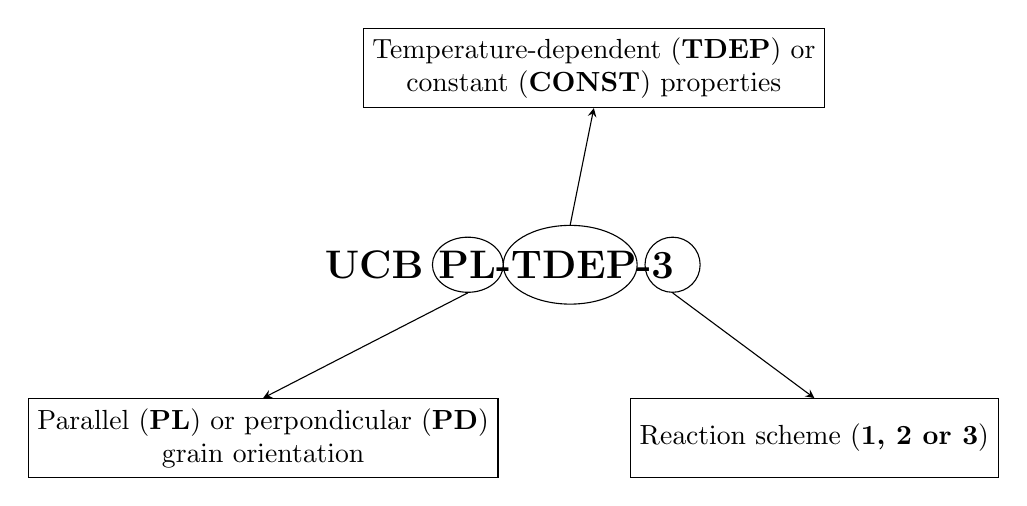
\begin{tikzpicture}[>=stealth]

% Texte principal
\node (ucb) at (0,0) {\Large \textbf{UCB PL-TDEP-3}};

% Ellipse autour de PL
\node[draw,ellipse,minimum width=0.9cm,minimum height=0.7cm]
(pl) at (-0.4,0) {};

% Ellipse autour de TDEP
\node[draw,ellipse,minimum width=1.7cm,minimum height=1.0cm]
(tdep) at (0.9,0) {};

% Ellipse autour de 3
\node[draw,ellipse,minimum width=0.7cm,minimum height=0.7cm]
(scheme) at (2.2,0) {};

% Boîte du haut
\node[
draw,
rectangle,
minimum width=4.5cm,
minimum height=1cm,
align=center
] (top) at (1.2,2.5)
{Temperature-dependent (\textbf{TDEP}) or \\ constant (\textbf{CONST}) properties};

% Boîte bas gauche
\node[
draw,
rectangle,
minimum width=4cm,
minimum height=1cm,
align=center
] (leftbox) at (-3,-2.2)
{Parallel (\textbf{PL}) or perpondicular (\textbf{PD})\\ grain orientation};

% Boîte bas droite
\node[
draw,
rectangle,
minimum width=4cm,
minimum height=1cm,
align=center
] (rightbox) at (4,-2.2)
{Reaction scheme (\textbf{1, 2 or 3})};

% Flèches
\draw[->] (pl.south) -- (leftbox.north);
\draw[->] (tdep.north) -- (top.south);
\draw[->] (scheme.south) -- (rightbox.north);

\end{tikzpicture}
\caption{Interpretation of the naming convention UCB-PL-TDEP-3.}
\label{fig:ucb-naming}
\end{figure}

\section{Results and discussion}

The objective of the MaCFP-4 condensed-phase benchmark exercise is to perform a model-to-model comparison. Since no common set of physical assumptions was imposed on the participants, and considering the diversity of the submitted modelling approaches, each contribution was treated as a separate model in the analysis. This approach makes it possible to assess the extent to which different modelling choices and assumptions affect the predicted results. Furthermore, the comparison of these contributions provides an opportunity to evaluate the individual influence of specific modelling assumptions on the simulation outcomes.

\subsection{TGA results}
The TGA results are evaluated based on two criteria: (i) the comparison of the mass loss rate (MLR) curves and (ii) the comparison of the peak MLR (\textbf{pMLR}) values together with their corresponding temperatures(\textbf{T\_pMLR}). The analysis is conducted for two simulated heating rates, 10 K/min and 100 K/min.\\

To compare the mass loss rate (MLR) predictions, the mass loss curves provided by the participating organizations were first differentiated to obtain the corresponding MLR curves. The resulting MLR data were then interpolated onto a common grid, enabling the calculation of the mean value (Eq. \ref{eq:mean_value}) and the standard deviation (Eq. \ref{eq:std_deviation}) at each point. In these equations, $x_i$ denotes the predicted value at a given time, $n$ is the number of predictions, $\bar{x}$ (or $Mean$) represents the mean value, and $Std$ denotes the standard deviation. The purpose of calculating the mean value and its associated standard deviation is to quantify the degree of agreement among the different model predictions. A low standard deviation indicates a strong consistency between the models, whereas a high standard deviation reflects a greater spread in the predictions and, therefore, a lower level of agreement among the participants.

\begin{equation} 
\bar{x} = \frac{1}{n}\sum_{i=1}^{n} x_i 
\label{eq:mean_value}
\end{equation}

\begin{equation} 
Std = \sqrt{ \frac{\sum_{i=1}^{n}\left(x_i-\bar{x}\right)^2} {n-1} } 
\label{eq:std_deviation}
\end{equation}

Figures \ref{fig:TGA_10K/min} and \ref{fig:TGA_100K/min} present the TGA mass loss rate (MLR) curves obtained for heating rates of 10 K/min and 100 K/min, respectively. The predictions for the 10 K/min case exhibit substantial discrepancies, with peak MLR values differing by up to one order of magnitude. Nevertheless, most predictions remain clustered within a relatively narrow range, while one contribution clearly deviates from the others, likely as a result of an error in the submitted data. To enable a more meaningful comparison, the 10 K/min analysis was repeated without this outlying contribution (Figure \ref{fig:TGA_100K/min_withoutFSRI}).

Excluding this dataset reveals an improved level of agreement among the remaining predictions, although noticeable differences still persist. These discrepancies may arise from the different modelling assumptions adopted by the participants, as well as from the experimental datasets selected for model calibration. Indeed, the experimental benchmark exercise, which included both TGA and gasification measurements, highlighted considerable variability among the submitted experimental results. Since the present modelling exercise relies directly on these experimental data, part of the observed variability in the predictions can reasonably be attributed to the variability already present in the benchmark measurements themselves.

The results obtained for the 100 K/min heating rate exhibit even larger discrepancies among the different contributions. The predicted peak MLR values vary by nearly a factor of two between the lowest and highest predictions. This behaviour may be explained by the same two factors discussed previously, namely differences in modelling assumptions and differences in the experimental datasets used for model calibration. It is also worth noting that the discrepancies observed in the experimental benchmark data become more pronounced at higher heating rates. Since the present modelling exercise is directly based on these experimental measurements, part of the variability observed in the predictions at 100 K/min is likely inherited from the increased uncertainty and scatter in the underlying experimental data. 

\begin{figure}[htbp]
    \centering
    \includegraphics[width=0.8\textwidth]{TGA_figures/TGA_10K-min.png}
    \caption{Predicted TGA MLR at 10 K/min.}
    \label{fig:TGA_10K/min}
\end{figure}

\begin{figure}[htbp]
    \centering
    \includegraphics[width=0.8\textwidth]{TGA_figures/TGA_100K-min.png}
    \caption{Predicted TGA MLR at 100 K/min.}
    \label{fig:TGA_100K/min}
\end{figure}

\begin{figure}[htbp]
    \centering
    \includegraphics[width=0.8\textwidth]{TGA_figures/TGA_10K-min_withoutFSRI.png}
    \caption{Predicted TGA MLR at 10 K/min (reproduction of Figure \ref{fig:TGA_10K/min} excluding singular behavior shown by one contribution).}
    \label{fig:TGA_100K/min_withoutFSRI}
\end{figure}

Table \ref{tab:TGA_stats} summarizes the mean values and standard deviations of the predicted peak mass loss rates (pMLR) and the corresponding peak temperatures. An interesting observation is that all participants predicted very similar temperatures at peak MLR, with a standard deviation of less than 1\% for both heating rates. In contrast, the variability in the predicted pMLR values is much larger, particularly for the 10 K/min case.

This high standard deviation at 10 K/min is primarily driven by the singular behaviour of one contribution discussed previously. When this outlying prediction is excluded from the analysis, the standard deviation of the pMLR decreases significantly, indicating a better agreement among the remaining contributions.

Overall, these results are encouraging, especially considering the complexity of the material behaviour and the significant scatter observed in the experimental data used as the basis for model calibration. The close agreement in the predicted peak temperatures, together with the improved consistency in pMLR predictions after removal of the apparent outlier, suggests that the participating models capture the main features of the thermal degradation process in a relatively consistent manner.  

\begin{table}[htbp] 
\centering 
\caption{Statistical summary of the predicted TGA peak mass loss rate (pMLR) and corresponding temperature.} 
\label{tab:TGA_stats} 
\begin{tabular}{lcccc} 
\toprule & \multicolumn{2}{c}{10 K/min} & \multicolumn{2}{c}{100 K/min} \\ \cmidrule(lr){2-3} \cmidrule(lr){4-5} & pMLR (g/s) & $T_{\mathrm{pMLR}}$ (K) & pMLR (g/s) & $T_{\mathrm{pMLR}}$ (K) \\ 
\midrule 
Mean value & 0.014 & 635 & 0.061 & 685 \\ 
Standard deviation (\%) & 121 & 1 & 23 & 1 \\ \bottomrule 
\end{tabular} 
\end{table}

\subsection{Gasification results (FPA simulations)}

The 1D gasification results are evaluated using the following two approaches: 
\begin{enumerate} 
\item Comparison of the mass loss rate (MLR) and back-surface temperature curves. 
\item Comparison of key characteristic quantities, namely the peak mass loss rate ($pMLR$), the time to peak mass loss rate ($t_{\mathrm{pMLR}}$), the onset time ($t_{\mathrm{onset}}$), and the end-of-pyrolysis time ($t_{\mathrm{end}}$). \end{enumerate} 

The analysis is performed for six simulation scenarios, corresponding to the combination of three external heat fluxes (10, 30, and 60~kW\,m$^{-2}$) and two sample thicknesses (6 and 18~mm). As discussed above, the various contributions provided by the participating organizations are considered as independent model predictions because they are based on different modelling assumptions, parameter sets, and calibration strategies. As a result, the present comparison comprises one model from CORIA, two models from UMD-FSRI, and twelve models from UCB.\\

Figures \ref{fig:FPA_MLR_q10_6mm} to \ref{fig:FPA_MLR_q60_18mm} present the predicted mass loss rate (MLR) curves for the different heat fluxes and sample thicknesses considered in this study. For each case, the ensemble mean prediction is shown together with a shaded region representing the standard deviation. 

Overall, the different models exhibit a consistent qualitative behaviour. At low heat fluxes, the predictions generally display a single dominant MLR peak, whereas a more pronounced double-peak behaviour emerges as the incident heat flux increases. This trend is observed for most contributions and is therefore reflected in the mean predictions. Since oxidation processes are not considered in the present simulations, the appearance of two distinct peaks cannot be attributed to char oxidation. Instead, it is likely related to the thermal decomposition of the different wood constituents and the development of temperature gradients within the sample. Hemicellulose typically decomposes at lower temperatures than cellulose, while lignin degrades over a much broader temperature range. As the heat flux increases, the heating rate becomes higher and these degradation stages may become more clearly separated in time, leading to the emergence of two distinct MLR peaks. In addition, the larger temperature gradients that develop within the material under higher thermal loads, together with the formation of a char layer at the surface, can further promote the separation of the dominant decomposition processes. The models also successfully predict an increase in the peak mass loss rate (MLR) and a reduction in fire duration with increasing heat flux. Conversely, increasing the material thickness is predicted to decrease the peak MLR while extending the fire duration.

\begin{figure}[htbp]
    \centering
    \includegraphics[width=0.8\textwidth]{FPA_figures/mlr_vs_t_q10_6mm.png}
    \caption{Predicted 1D gasification MLR: heat flux = 10 kW/m²; thickness = 6mm.}
    \label{fig:FPA_MLR_q10_6mm}
\end{figure}
\begin{figure}[htbp]
    \centering
    \includegraphics[width=0.8\textwidth]{FPA_figures/mlr_vs_t_q10_18mm.png}
    \caption{Predicted 1D gasification MLR: heat flux = 10 kW/m²; thickness = 18mm.}
    \label{fig:FPA_MLR_q10_18mm}
\end{figure}
\begin{figure}[htbp]
    \centering
    \includegraphics[width=0.8\textwidth]{FPA_figures/mlr_vs_t_q30_6mm.png}
    \caption{Predicted 1D gasification MLR: heat flux = 30 kW/m²; thickness = 6mm.}
    \label{fig:FPA_MLR_q30_6mm}
\end{figure}
\begin{figure}[htbp]
    \centering
    \includegraphics[width=0.8\textwidth]{FPA_figures/mlr_vs_t_q30_18mm.png}
    \caption{Predicted 1D gasification MLR: heat flux = 30 kW/m²; thickness = 18mm.}
    \label{fig:FPA_MLR_q30_18mm}
\end{figure}
\begin{figure}[htbp]
    \centering
    \includegraphics[width=0.8\textwidth]{FPA_figures/mlr_vs_t_q60_6mm.png}
    \caption{Predicted 1D gasification MLR: heat flux = 60 kW/m²; thickness = 6mm.}
    \label{fig:FPA_MLR_q60_6mm}
\end{figure}
\begin{figure}[htbp]
    \centering
    \includegraphics[width=0.8\textwidth]{FPA_figures/mlr_vs_t_q60_18mm.png}
    \caption{Predicted 1D gasification MLR: heat flux = 60 kW/m²; thickness = 18mm.}
    \label{fig:FPA_MLR_q60_18mm}
\end{figure}

Figures \ref{fig:FPA_Tback_q10_6mm} to \ref{fig:FPA_MLR_q60_18mm} present the back-surface temperature predicted by the different models under the various operating conditions. Similar to the mass loss rate (MLR) results, all models predict the same general trends. Specifically, the models predict an increase in the asymptotic back-surface temperature with increasing heat flux, accompanied by a shorter transient phase. Conversely, increasing the sample thickness results in a lower asymptotic temperature and a longer transient phase before steady-state conditions are reached. It is also worth noting that the models tend to produce more consistent predictions during the steady-state phase than during the transient phase. Another interesting observation is the overall better agreement between the models for the thinner samples compared to the thicker ones. A possible explanation is that increasing the sample thickness results in the formation of a thicker char layer, which enhances the influence of physical phenomena such as radiative heat transfer and mass transport within the porous char structure. Since these processes are modelled differently by the various models, larger discrepancies in the predictions can be expected for thicker samples.

The operating condition for which the agreement between the models is the poorest corresponds to the highest imposed heat flux combined with the greatest sample thickness. Identifying this critical scenario is particularly valuable, as it highlights the conditions under which the predictive capabilities of the models diverge the most. This observation suggests that further efforts should be directed toward improving the representation of thermally thick behaviours, which appear to be more challenging to predict accurately. The increased complexity of these conditions is likely associated with the larger temperature gradients, thicker char layers, and heat and mass transfer processes that develop within the material.\\


\begin{figure}[htbp]
    \centering
    \includegraphics[width=0.8\textwidth]{FPA_figures/T_back_vs_t_q10_6mm.png}
    \caption{Predicted back surface temperature: heat flux = 10 kW/m²; thickness = 6mm.}
    \label{fig:FPA_Tback_q10_6mm}
\end{figure}
\begin{figure}[htbp]
    \centering
    \includegraphics[width=0.8\textwidth]{FPA_figures/T_back_vs_t_q10_18mm.png}
    \caption{Predicted back surface temperature: heat flux = 10 kW/m²; thickness = 18mm.}
    \label{fig:FPA_Tback_q10_18mm}
\end{figure}
\begin{figure}[htbp]
    \centering
    \includegraphics[width=0.8\textwidth]{FPA_figures/T_back_vs_t_q30_6mm.png}
    \caption{Predicted back surface temperature: heat flux = 30 kW/m²; thickness = 6mm.}
    \label{fig:FPA_Tback_q30_6mm}
\end{figure}
\begin{figure}[htbp]
    \centering
    \includegraphics[width=0.8\textwidth]{FPA_figures/T_back_vs_t_q30_18mm.png}
    \caption{Predicted back surface temperature: heat flux = 30 kW/m²; thickness = 18mm.}
    \label{fig:FPA_Tback_q30_18mm}
\end{figure}
\begin{figure}[htbp]
    \centering
    \includegraphics[width=0.8\textwidth]{FPA_figures/T_back_vs_t_q60_6mm.png}
    \caption{Predicted back surface temperature: heat flux = 60 kW/m²; thickness = 6mm.}
    \label{fig:FPA_Tback_q60_6mm}
\end{figure}
\begin{figure}[htbp]
    \centering
    \includegraphics[width=0.8\textwidth]{FPA_figures/T_back_vs_t_q60_18mm.png}
    \caption{Predicted back surface temperature: heat flux = 60 kW/m²; thickness = 18mm.}
    \label{fig:FPA_Tback_q60_18mm}
\end{figure}

In order to have a more quantitative comparison, figures \ref{fig:FPA_onset_time_stats}, \ref{fig:FPA_peak_MLR_stats}, \ref{fig:FPA_t_peak_MLR_stats} and \ref{fig:FPA_t_end_stats} represent the  predicted mean onset time, the predicted mean MLR, the predicted mean time to peak MLR and the predicted mean end-of-pyrolysis time, respectively. The associated standard deviation to the mean value is represented by the error bars. The mean value and standard deviation are calculated for each parameter, using equation \ref{eq:mean_value} and \ref{eq:std_deviation}. 
These values are also presented on table \ref{tab:FPA_stats_results}. 

Regarding $t_{pMLR}$, the relative standard deviation exhibits contrasting behavior with increasing heat flux depending on the sample thickness. For the thinner samples, it decreases slightly as the heat flux increases and remains relatively low, with values below 20\%. In contrast, for the thicker samples, the relative standard deviation increases with heat flux, reaching values as high as 63.9\%, before decreasing slightly at the highest heat flux levels. For $pMLR$, the opposite trend is observed: the relative standard deviation increases with heat flux for the thinner samples and decreases for the thicker ones. Nevertheless, the variability remains within an acceptable range, with values around 20\%. 
The relative standard deviations of both $t_{onset}$ and $t_{end}$ increase with increasing heat flux, irrespective of sample thickness. It is important to note, however, that the mean value of $t_{onset}$ decreases markedly as the heat flux increases, approaching nearly instantaneous onset times. Under these conditions, even small absolute variations can result in large relative standard deviations. This increased sensitivity to experimental uncertainties likely explains the observed rise in variability at higher heat fluxes.It is also noteworthy that the relative standard deviations associated with these two parameters are particularly high, reaching up to 45.5\% for $t_{onset}$ and 68.7\% for $t_{end}$. These values reveal a substantial scatter in the models' predictions. Overall, the comparison of the different pyrolysis characteristics indicates that $pMLR$, and to a lesser extent $t_{pMLR}$, are more predictable parameters. In contrast, $t_{onset}$ and $t_{end}$ display larger variability, highlighting their greater sensitivity to models' assumptions. Finally, the results associated with the end-of-pyrolysis time, $t_{end}$, for the 18 mm sample should be treated with caution, since some simulations were stopped before the completion of the pyrolysis process.

\begin{figure}[htbp]
    \centering
    \includegraphics[width=0.8\textwidth]{FPA_figures/onset_time.png}
    \caption{Predicted mean onset time and associated standard deviation in function of heat flux.}
    \label{fig:FPA_onset_time_stats}
\end{figure}
\begin{figure}[htbp]
    \centering
    \includegraphics[width=0.8\textwidth]{FPA_figures/peak_mlr.png}
    \caption{Predicted mean peak MLR and associated standard deviation in function of heat flux.}
    \label{fig:FPA_peak_MLR_stats}
\end{figure}
\begin{figure}[htbp]
    \centering
    \includegraphics[width=0.8\textwidth]{FPA_figures/time_to_peak_mlr.png}
    \caption{Predicted mean time to peak MLR and associated standard deviation in function of heat flux.}
    \label{fig:FPA_t_peak_MLR_stats}
\end{figure}
\begin{figure}[htbp]
    \centering
    \includegraphics[width=0.8\textwidth]{FPA_figures/final_time.png}
    \caption{Predicted mean end-of-pyrolysis time and associated standard deviation in function of heat flux.}
    \label{fig:FPA_t_end_stats}
\end{figure}


\begin{table*}[htbp] 
\centering
\caption{Mean values and relative standard deviations (RSD) of the characteristic fire parameters.} \label{tab:FPA_stats_results} 
\small 
\begin{tabular}{lcccccccc} 
\toprule 
& \multicolumn{2}{c}{$t_{pMLR}$ (s)} 
& \multicolumn{2}{c}{$pMLR$ (g\,m$^{-2}$\,s$^{-1}$)} 
& \multicolumn{2}{c}{$t_{onset}$ (s)} 
& \multicolumn{2}{c}{$t_{end}$ (s)} \\ 
\cmidrule(lr){2-3} 
\cmidrule(lr){4-5} 
\cmidrule(lr){6-7} 
\cmidrule(lr){8-9} 
Case & Mean $\pm$ SD & RSD (\%) 
     & Mean $\pm$ SD & RSD (\%) 
     & Mean $\pm$ SD & RSD (\%) 
     & Mean $\pm$ SD & RSD (\%) \\ 
\midrule 
q10\_6mm &
$468 \pm 72$ &
15.4 &
$2.96 \pm 0.49$ &
16.6 &
$213 \pm 26$ &
12.3 &
$1884 \pm 586$ &
31.1 \\ 

q10\_18mm &
$1927 \pm 368$ &
19.1 &
$2.24 \pm 0.47$ &
20.8 &
$717 \pm 134$ &
18.7 &
$3206 \pm 515$ &
16.1 \\ 

q30\_6mm &
$176 \pm 18$ &
10.4 &
$11.74 \pm 2.42$ &
20.7 &
$24 \pm 12$ &
50.6 &
$646 \pm 223$ &
34.6 \\ 

q30\_18mm &
$554 \pm 354$ &
63.9 &
$6.22 \pm 1.09$ &
17.5 &
$24 \pm 11$ &
46.0 &
$1685 \pm 505$ &
29.9 \\ 

q60\_6mm &
$108 \pm 14$ &
12.5 &
$19.26 \pm 4.38$ &
22.7 &
$7 \pm 5$ &
68.7 &
$480 \pm 218$ &
45.5 \\ 

q60\_18mm &
$21 \pm 12$ &
55.3 &
$13.39 \pm 1.68$ &
12.6 &
$6 \pm 3$ &
50.6 &
$1187 \pm 423$ &
35.7 \\ 
\bottomrule 
\end{tabular} 
\end{table*}

\subsubsection{Sensitivity Analysis of Individual Physical Assumptions} 

The UCB contribution provides a valuable dataset for assessing the influence of key modeling assumptions on gasification predictions. Three classes of assumptions were investigated: 

\begin{enumerate} 
\item Thermophysical properties: temperature-dependent properties (\textit{TDEP}) versus constant properties (\textit{CONST}); 
\item Fiber orientation: parallel (\textit{PL}) versus perpendicular (\textit{PD}) orientation with respect to the exposed surface; 
\item Kinetic scheme: three different kinetic mechanisms were considered, as described in the previous section. \end{enumerate} 

The availability of these simulations enables a sensitivity analysis of these assumptions on the main characteristics of the mass-loss-rate (MLR) curve. A key advantage of this simulation dataset is that it isolates the impact of individual modeling assumptions while keeping all other model components unchanged. In particular, aspects that are outside the scope of this benchmark, such as radiation modeling and heat and mass transfer within porous media, remain identical across all simulations. The objective is therefore to quantify the influence of each modeling assumption on four key quantities of interest, including the onset time ($t_{\mathrm{onset}}$), peak MLR ($pMLR$), time to peak MLR ($t_{\mathrm{pMLR}}$). The parameter $t_{end}$ is not included in this comparison since an important part of the simulation were stopped before the pyrolysis ended.

For each test case, the influence of a given assumption was isolated by comparing pairs of simulations that differed only in the assumption under investigation, while all other modeling parameters were kept unchanged. The impact of the assumption was quantified using a symmetric relative error, and the corresponding mean value and standard deviation were subsequently computed. As an example, for the q=10 kW/m² and 6mm case, the effect of thermophysical properties was evaluated by comparing \textit{TDEP} and \textit{CONST} simulations while keeping both the kinetic mechanism and the fiber orientation identical. The same methodology was applied to assess the influence of fiber orientation and kinetic parameters across all heat-flux and thickness conditions considered in the benchmark.

Table~\ref{tab:sensitivity_flux_thickness} presents the mean relative errors and associated standard deviations obtained for the different modeling assumptions and operating conditions. The standard deviation of the relative error for $t_{onset}$, $pMLR$ and $t_{pMLR}$ is plotted as a function of the external heat flux for both sample thicknesses 6mm and 18mm in Figures~\ref{fig:FPA_CONST_vs_TDEP}, \ref{fig:FPA_PL_vs_PD}, and \ref{fig:FPA_kin_effect}. These figures highlight the influence of the thermophysical-property formulation (\textit{CONST} vs.\ \textit{TDEP}), fiber orientation (\textit{PL} vs.\ \textit{PD}), and the kinetic scheme on the predicted characteristics of the MLR curve, respectively. The observations from these figures and the accompanying table indicate that the influence of the different modeling assumptions depends strongly on the heat flux and material thickness being considered. Furthermore, the impact of these assumptions varies according to the quantity of interest under investigation. Another noteworthy observation is that the effects of the modeling assumptions are not monotonic. In other words, increasing the heat flux or the thickness does not necessarily lead to a consistent increase or decrease in the influence of a given assumption. This behavior highlights the complexity of the underlying physical processes and the strong interactions between the model physics and the characteristics of the studied scenario, namely the imposed heat flux and material thickness.\\

Accounting for the temperature dependence of the thermophysical properties affects the peak mass-loss rate differently depending on the sample thickness. For the thin sample, the influence of this assumption increases with increasing heat flux, whereas the opposite trend is observed for the thick sample. Overall, the impact of this assumption on $pMLR$ remains moderate, with variations below 20\%. Regarding $t_{pMLR}$, this assumption has almost no influence on the thin sample, whereas its effect can reach up to 80\% for the thick sample, which is substantial. The onset time, $t_{onset}$, is also affected by this assumption. Its influence is limited at low heat fluxes but can increase up to 27\% for the thick sample exposed to the highest heat flux.\\

It is interesting to note the strong similarity between the trends associated with the influence of fiber orientation and those associated with the temperature dependence of the thermophysical properties on the various characteristics of the MLR curve. It is important, however, to keep in mind that the mean values of the quantities of interest differ between the two cases, and that the corresponding absolute values of the standard deviations are also different. Nevertheless, the similarity in the observed trends, combined with the comparable ranges of standard deviation, suggests that both assumptions affect the model through a common underlying mechanism. A possible explanation is that assuming either a parallel or a perpendicular fiber orientation effectively corresponds to considering different thermophysical properties governing heat transfer within the solid. As a result, modifications induced by the fiber orientation assumption primarily alter the conductive heat transfer behavior, in a manner analogous to the temperature dependence of the thermophysical properties. Consequently, both assumptions influence the thermal response of the material through closely related physical mechanisms, which may explain the observed similarities in their effects on the MLR curve characteristics.\\

The influence of the kinetic mechanism on the MLR curve characteristics is generally moderate, although its impact varies significantly with both heat flux and sample thickness. For $pMLR$, the effect remains relatively limited, with standard deviations below 16\% in all cases. For the thin sample, the influence tends to increase with heat flux, rising from approximately 11\% at 10 kW/m$^2$ to more than 15\% at 60 kW/m$^2$. By contrast, for the thick sample, the influence decreases with increasing heat flux and becomes almost negligible at 60 kW/m$^2$. Regarding $t_{pMLR}$, the kinetic mechanism has a relatively small influence on the thin sample. However, its impact becomes much more pronounced for the thick sample. In particular, at 30 kW/m$^2$. This trend is remarkably similar to that observed for the temperature dependence of the thermophysical properties. The onset time, $t_{onset}$, appears to be one of the most sensitive quantities to the kinetic mechanism. For both thicknesses, the influence generally increases with heat flux. For the thin sample, the standard deviation increases from about 20\% to more than 25\% between 10 and 60 kW/m$^2$. A similar behavior is observed for the thick sample, for which the maximum influence reaches approximately 28\% at 30 kW/m$^2$. These results indicate that the kinetic mechanism plays an important role in controlling the initiation of thermal degradation. Overall, the kinetic mechanism primarily affects the temporal characteristics of the MLR curve rather than its magnitude. In particular, its strongest influence is observed on $t_{pMLR}$ and $t_{onset}$ for the thick sample, highlighting the important role played by the decomposition kinetics in controlling the progression of thermal degradation within the material.

Interestingly, the influence of the kinetic mechanism exhibits trends that are qualitatively similar to those observed for the temperature dependence of the thermophysical properties. In particular, both assumptions have a limited effect on $pMLR$ but can strongly affect $t_{pMLR}$ and $t_{onset}$ for thick samples. This similarity suggests that both assumptions modify the balance between heat transfer and decomposition processes, although through different physical pathways. While the temperature-dependent properties primarily alter heat penetration within the solid, the kinetic mechanism directly controls the rate at which the material decomposes once sufficient thermal energy has been accumulated.\\

\begin{table*}[htbp] \centering \caption{Sensitivity of the main MLR characteristics to the investigated modeling assumptions. Values correspond to the mean relative error (\%) $\pm$ standard deviation.} \label{tab:sensitivity_flux_thickness} \resizebox{\textwidth}{!}{ \begin{tabular}{llccc} \hline \textbf{Hypothesis} & \textbf{Case} & \textbf{$pMLR$ (\%)} & \textbf{$t_{\mathrm{pMLR}}$ (\%)} & \textbf{$t_{\mathrm{onset}}$ (\%)} \\ \hline CONST vs TDEP & $q10$--6 mm & 31.3 $\pm$ 10.7 & 20.9 $\pm$ 13.9 & 15.3 $\pm$ 11.8 \\ CONST vs TDEP & $q30$--6 mm & 24.9 $\pm$ 16.6 & 19.1 $\pm$ 12.1 & 15.9 $\pm$ 10.3 \\ CONST vs TDEP & $q60$--6 mm & 17.7 $\pm$ 20.4 & 17.3 $\pm$ 14.6 & 15.9 $\pm$ 27.4 \\ CONST vs TDEP & $q10$--18 mm & 28.4 $\pm$ 15.5 & 22.3 $\pm$ 14.6 & 15.9 $\pm$ 11.2 \\ CONST vs TDEP & $q30$--18 mm & 13.0 $\pm$ 12.7 & 67.2 $\pm$ 81.3 & 24.3 $\pm$ 21.4 \\ CONST vs TDEP & $q60$--18 mm & 16.5 $\pm$ 4.8 & 33.5 $\pm$ 20.4 & 17.9 $\pm$ 21.1 \\ \hline Kinetic scheme & $q10$--6 mm & 11.1 $\pm$ 7.2 & 10.9 $\pm$ 10.5 & 20.4 $\pm$ 14.4 \\ Kinetic scheme & $q30$--6 mm & 11.9 $\pm$ 12.8 & 7.3 $\pm$ 6.7 & 21.1 $\pm$ 15.5 \\ Kinetic scheme & $q60$--6 mm & 15.1 $\pm$ 14.6 & 9.8 $\pm$ 10.9 & 25.4 $\pm$ 23.4 \\ Kinetic scheme & $q10$--18 mm & 14.1 $\pm$ 11.1 & 16.1 $\pm$ 14.8 & 21.1 $\pm$ 15.5 \\ Kinetic scheme & $q30$--18 mm & 9.5 $\pm$ 8.8 & 61.9 $\pm$ 79.3 & 27.6 $\pm$ 23.6 \\ Kinetic scheme & $q60$--18 mm & 3.9 $\pm$ 3.5 & 22.2 $\pm$ 12.6 & 17.9 $\pm$ 20.1 \\ \hline PL vs PD & $q10$--6 mm & 6.9 $\pm$ 6.5 & 8.7 $\pm$ 8.5 & 12.1 $\pm$ 12.6 \\ PL vs PD & $q30$--6 mm & 27.9 $\pm$ 16.6 & 9.3 $\pm$ 2.8 & 12.8 $\pm$ 8.5 \\ PL vs PD & $q60$--6 mm & 40.0 $\pm$ 20.8 & 16.0 $\pm$ 11.3 & 16.2 $\pm$ 18.2 \\ PL vs PD & $q10$--18 mm & 19.3 $\pm$ 16.0 & 13.2 $\pm$ 13.2 & 12.8 $\pm$ 13.9 \\ PL vs PD & $q30$--18 mm & 30.6 $\pm$ 13.6 & 114.0 $\pm$ 85.6 & 21.1 $\pm$ 14.4 \\ PL vs PD & $q60$--18 mm & 12.0 $\pm$ 4.5 & 35.3 $\pm$ 17.6 & 8.5 $\pm$ 13.3 \\ \hline \end{tabular} } \end{table*}


\begin{figure}[htbp]
\centering 
\includegraphics[width=0.8\textwidth]{FPA_figures/CONST_vs_TDEP_2x2.png} 
\caption{Sensitivity of the predicted gasification characteristics to the treatment of thermophysical properties (\textit{CONST} vs.\ \textit{TDEP}). The standard deviation of the relative error associated with $t_{onset}$, ${pMLR}$ and $t_{pMLR}$) is shown as a function of the external heat flux for the two sample thicknesses (6mm and 18mm).} 
\label{fig:FPA_CONST_vs_TDEP}
\end{figure}
\begin{figure}[htbp]
\centering 
\includegraphics[width=0.8\textwidth]{FPA_figures/PL_vs_PD_2x2.png} 
\caption{Sensitivity of the predicted gasification characteristics to the fibers' orientation (\textit{PL} vs.\ \textit{PD}).The standard deviation of the relative error associated with $t_{onset}$, ${pMLR}$ and $t_{pMLR}$) is shown as a function of the external heat flux for the two sample thicknesses (6mm and 18mm).} 
\label{fig:FPA_PL_vs_PD}
\end{figure}
\begin{figure}[htbp]
\centering 
\includegraphics[width=0.8\textwidth]{FPA_figures/KINETIC_EFFECT_2x2.png} 
\caption{Sensitivity of the predicted gasification characteristics to the kinetic mechanism. The standard deviation of the relative error associated with $t_{onset}$, ${pMLR}$ and $t_{pMLR}$) is shown as a function of the external heat flux for the two sample thicknesses (6mm and 18mm).} 
\label{fig:FPA_kin_effect}
\end{figure}



\FloatBarrier
\section{Conclusion}

The comparison of the different models highlights a good overall agreement in terms of qualitative predictions. All models reproduce similar trends for both TGA and 1D gasification simulations, providing encouraging results and confirming their ability to capture the main physical and kinetic phenomena. However, significant quantitative discrepancies remain. These differences can be attributed to variations in model assumptions, including the initial pine wood composition, fiber orientation, reaction mechanisms, thermophysical properties, and kinetic parameters. In particular, the use of different experimental datasets and calibration procedures for kinetic parameter identification contributes to the observed discrepancies. The results also indicate that the magnitude of these discrepancies depends on the operating conditions, such as the imposed heat flux, sample thickness, and the quantity of interest. Under certain conditions, the predictions converge and provide close estimates, whereas under others, phenomena such as radiative heat transfer, porous medium effects, or thermally thin/thick behavior become more influential. Overall, the study suggests that the observed differences are primarily driven by modeling assumptions and input data rather than by the numerical framework itself. Future work should focus on validation in order to complete the analysis.

\FloatBarrier
\bibliographystyle{plain}
\bibliography{sample}

\end{document}
